\documentclass[14pt,a4paper]{scrartcl}
\usepackage[left=1.5cm,right=1.5cm,
    top=1.5cm,bottom=1cm,bindingoffset=0cm]{geometry}

\usepackage[T1,T2A]{fontenc}
\usepackage[utf8]{inputenc}
\usepackage[english,russian,ukrainian]{babel}
\usepackage{tabularx}
\usepackage{amssymb}
\usepackage{color}
\usepackage{amsmath}
\usepackage{mathrsfs}
\usepackage{listings}
\usepackage{graphicx}
\graphicspath{ {./images/} }
%\usepackage{draftwatermark} не будет лезть на картинки
\usepackage[printwatermark]{xwatermark}%будет лезть на картинки
\usepackage{lipsum}
\usepackage{xcolor}
\usepackage{tikz}

 \usepackage{csvsimple}
 \usepackage{supertabular}
\usepackage{pdflscape}
\usepackage{fancyvrb}
\usepackage{comment}


\definecolor{ggreen}{rgb}{0.,1,0}
\begin{document}
\pagecolor{white}
\begin{titlepage}
  \begin{center}
    \large
    Національний технічний університет України \\ "Київський політехнічний інститут імені Ігоря Сікорського"


    Факультет Електроніки

    Кафедра мікроелектроніки
    \vfill

    \textsc{ЗВІТ}\\

    {\Large Про виконання контрольної роботи\\
      з дисципліни: «Технологічні основи електроніки»\\[1cm]



    }
  \bigskip
\end{center}
\vfill

\newlength{\ML}
\settowidth{\ML}{«\underline{\hspace{0.4cm}}» \underline{\hspace{2cm}}}
\hfill
\begin{minipage}{1\textwidth}
Виконавець:\\
Студент 3-го курсу \hspace{4cm} $\underset{\text{(підпис)}}{\underline{\hspace{0.2\textwidth}}}$  \hspace{1cm}А.\,С.~Мнацаканов\\
\vspace{1cm}

Превірив: \hspace{6.1cm} $\underset{\text{(підпис)}}{\underline{\hspace{0.2\textwidth}}}$  \hspace{1cm}О.\,В.~Мачулянський\\

\end{minipage}

\vfill

\begin{center}
2020
\end{center}
\end{titlepage}

%---------------------------------------------------------------------------------------------------------------------------------------------------------------------------------





\begin{center}1. ЗАВДАННЯ\\ \end{center}

\fcolorbox{black}{ggreen}{1}.Опишіть технологічний маршрут формування напівпровідникових
біполярних структур на прикладі планарно- епітаксіального біполярного
транзистора з ізоляцією зворотньо зміщеним р- п переходом.\par
\fcolorbox{black}{ggreen}{2}. Які основні домішки, використовують для створення шарів з донорною
провідністю в ІМС?\par
\fcolorbox{black}{ggreen}{3}. Який метод легування дозволяє формувати тонкі леговані шари з
концентрацією домішок вище їх граничної розчинності в напівпровіднику.\par
\fcolorbox{black}{ggreen}{4}. Сформулювати умови одержання легованих шарів методом
високотемпературної дифузії.\par
\fcolorbox{black}{ggreen}{5}. Які механізми дифузії найбільш вигідні в кремнії для домішок третьої та
п’ятої груп.\par
\fcolorbox{black}{ggreen}{6}. За допомогою яких параметрів можна керувати технологічним процесом
високотемпературної дифузії.\par
\fcolorbox{black}{ggreen}{7}. Який процес являється контрольною стадією при поліруючому хімічному
травленні.\par
\fcolorbox{black}{ggreen}{8}. Наведіть графік розподілу концентрації домішок в напівпровіднику при
двостадійній високотемпературній дифузії на етапі розгонки.\par
\fcolorbox{black}{ggreen}{9}. Які матеріали використовують в якості активного газу в технологічному
процесі плазмохімічного травлення.\par
Вибрати: $H_2 , CF_4, CO_2 , N_2 , Ar , He , O_2 , H_2S , HBr$.\par
\fcolorbox{black}{ggreen}{10}.  Від яких параметрів залежить швидкість процесу при хімічному
селективному травленні.\par
Вибрати: D – коефіцієнт дифузії реагенту; Nоб – концентрація\par
реагенту в об’ємі; Nпов – концентрація реагенту на поверхні; $\delta$--
товщина приповерхневого шару травника, в якому існує градієнт
концентрації; $N_A$ – концентрації реагуючих речовин; $\triangle E_a$ --енергія
активації хімічної решітки; Т – температура.\par

\fcolorbox{black}{ggreen}{11}. Які технологічні операції (назвати не менш трьох) при виготовленні ІМС
проводяться при температурі понад $1000^{\circ}С$?

\newpage
\begin{center}2.ВІДПОВІДІ\\ \end{center}


%---------------------------------------------------------------------------------------------------------------------------------------------------------------------------------

\fcolorbox{black}{ggreen}{1}
\begin{figure}[h]
\center{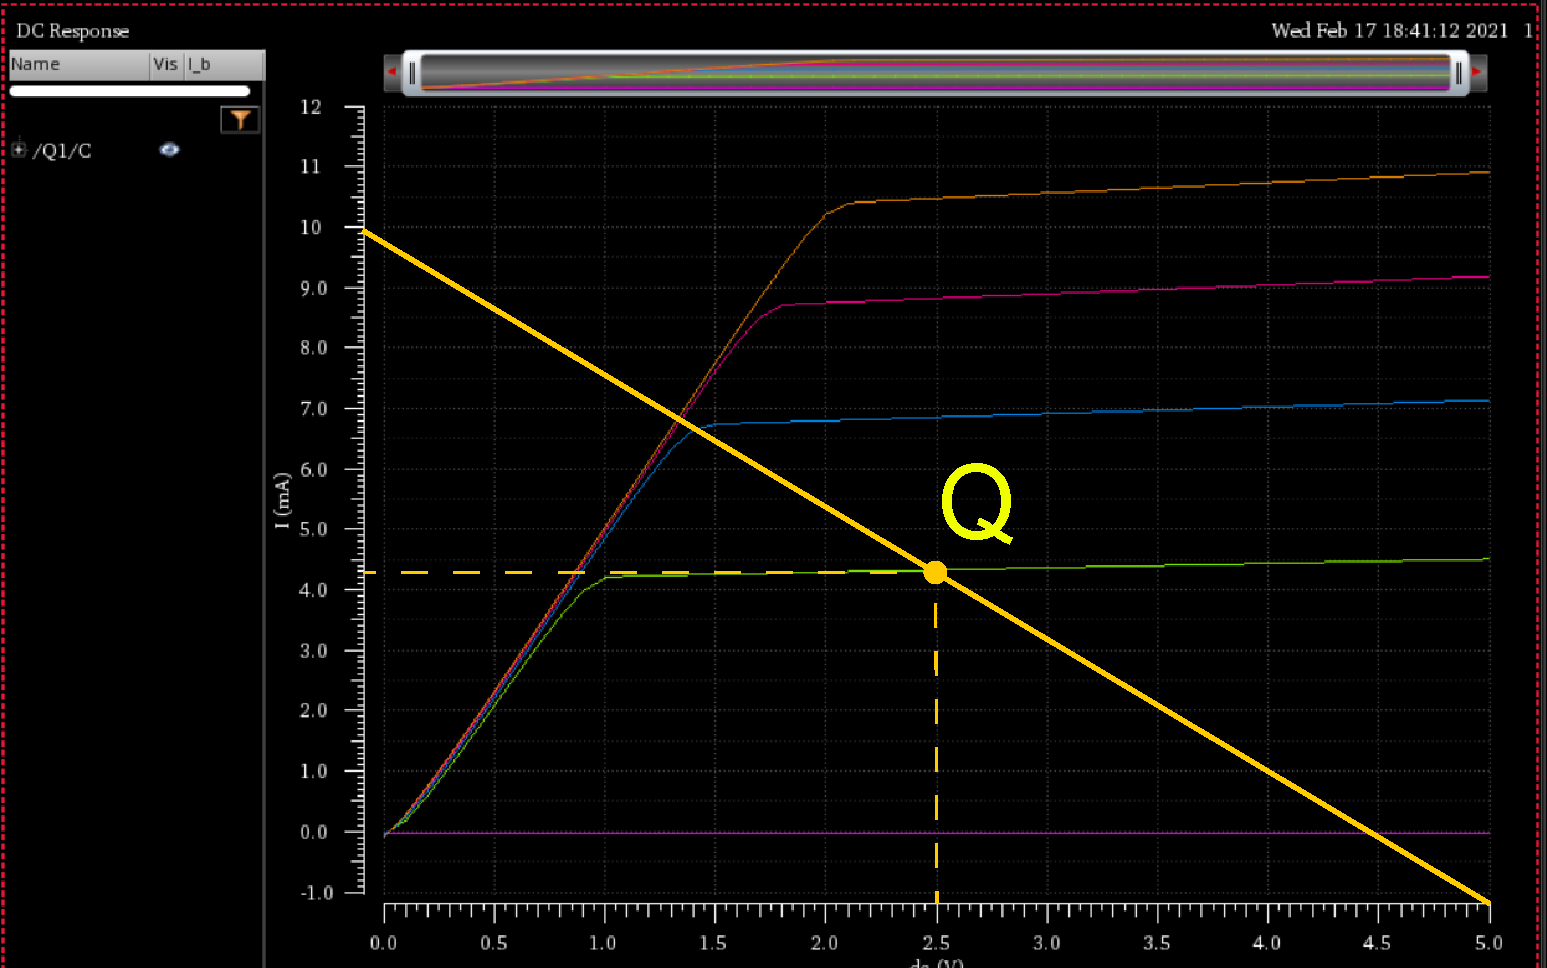
\includegraphics[width=0.9\linewidth]{1.png}}\\
\caption{Класифікація окремих технологічних процесів напівпровідникового виробництва .}
\end{figure}

\fcolorbox{black}{ggreen}{2}
Арсенід ($As$), Фосфор ($P$), Стибідій ($Sb$). 

\fcolorbox{black}{ggreen}{3}
Метод іонної імплантації\par
\fcolorbox{black}{ggreen}{4}
Необхідна (обов’язкова) умова: висока густина вакансій в напівпровіднику.\par

Достатня умова: Атом домішки в кристалі здатний генерувати вільний носій заряду (електрон або дірку) лише в тому випадку, якщо він займає місце у вузлі кристалічної решітки.\\

\fcolorbox{black}{ggreen}{5}
Їх може бути декілька: дифузія реагенту до поверхні або ще як варіант поверхнева хімічна реакція (визначається видом травника).\par
\fcolorbox{black}{ggreen}{6}
Приповерхнева концентрація, час дифузії, $t^{\circ}$
\fcolorbox{black}{ggreen}{7}
\newpage
\fcolorbox{black}{ggreen}{8}
\begin{figure}[h!]
\center{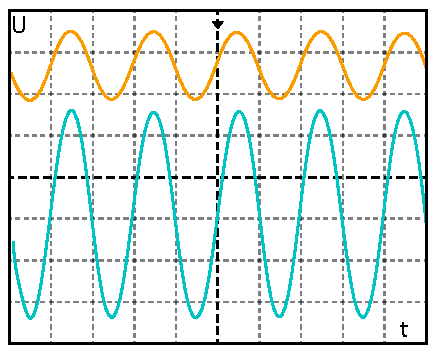
\includegraphics[width=0.9\linewidth]{8.png}}\\
\caption{Графіки розподілу концентрації домішки в напівпровіднику при дифузії з нескінченного(зліва) та обмеженего(зправа) джерел.}
\end{figure}

\fcolorbox{black}{ggreen}{9}
Окрім газів для ВПТ використовують пари токсичних рідин: $SiHCl_3$, $SiCl_4$, $CCl_4$, а також
суміші $HF, H_2S, NO, NF_3$ також $CF4$, але якщо додати кисень( $O_2$) –травлення піде швидше.\\
\fcolorbox{black}{ggreen}{10}
D – коефіцієнт дифузії реагенту $N_A$ – концентрації реагуючих речовин; $\triangle E_a$ --енергія
активації хімічної решітки; Т – температура\\
\fcolorbox{black}{ggreen}{11}
Високотемпературна дифузія, хлорне, хімічне травлення, термічне окиснення. 






%1---------------------------------------------------------------------------------------------------------------------------------------------------------------------------------









\end{document}